\documentclass[10pt]{article}

\usepackage[margin=.6in,footskip=0.58in,top=0.58in]{geometry}
\usepackage{natbib}
\usepackage{parskip}
\usepackage{graphicx}
\usepackage{titling}
\usepackage{multicol,caption}
\usepackage[hidelinks]{hyperref}
\bibliographystyle{abbrv}
\graphicspath{{./images/}}

\newenvironment{Figure}
  {\par\medskip\noindent\minipage{\linewidth}}
  {\endminipage\par\medskip}

\renewcommand\maketitlehooka{\null\mbox{}\vfill}
\renewcommand\maketitlehookd{\vfill\null}

\newcommand{\fontsmall}{\fontsize{8pt}{9pt}\selectfont}

\title{Active Learning of Feasible Region for Porous Ceramics}
\date{\today}
\author{Liam Latour}

\begin{document}

\begin{titlingpage}
\maketitle
\end{titlingpage}

\pagebreak

\section{Introduction}
\begin{multicols}{2}

Ceramic resin composites are advanced materials that combine the strength of ceramics with the flexibility of resins, resulting in enhanced durability and versatility. These composites are created by infusing porous ceramic structures with resin, achieving an impressive balance of properties that is vital for challenging environments. They are manufactured using techniques such as sintering\cite{leriche_sintering_2017} or additive manufacturing and undergo processes like vacuum impregnation or resin transfer molding to ensure homogeneity and reinforce the structure with increased toughness and ductility. These composites have wide-ranging applications across industries, including aerospace, automotive, and medical, as they enable the development of lightweight yet high-performance components.

To produce the porous ceramic using sintering\cite{ha_effect_2013}, porogens, often in the form of plastic beads, are mixed with the ceramic powder and subjected to pressure. The porogens are then eliminated through heating, ideally resulting in a porous, cohesive ceramic matrix. This matrix is subsequently sintered to solidify it before resin infusion.

Fluid transfer through materials is a critical process in numerous scientific and industrial applications, with the material's microstructure significantly influencing its efficiency. To better understand and predict the relationship between microstructure and fluid transfer, there is an increasing need for extensive microstructure databases. The porogen size distribution and total volume significantly impact the final material's porosity and, consequently, the resin-to-ceramic ratio. However, an excessive amount of porogens can cause the material to break before sintering, making it unusable. Determining the feasible region, i.e., the porogen mix that will not break, is essential for efficient manufacturing.

The feasible region is identified by testing samples with various porogen distributions. Unfortunately, each test is time-consuming, making blind exploration ineffective. Active learning, a subfield of machine learning, addresses this issue by optimizing the selection of candidate samples to be tested, thereby improving the model more efficiently. This article focuses on implementing an active learning strategy in the context of sparse data with continuous feature space.

% \begin{Figure}
%   \begin{tabular}{cc}
%     \includegraphics[width=0.5\columnwidth]{porogen_1.png} &   \includegraphics[width=0.5\columnwidth]{porogen_2.jpg} \\
%     \includegraphics[width=.5\columnwidth]{porogen_3.jpg} \\
%   \end{tabular}
%   \captionof{figure}{Sample images of porous ceramics}
% \end{Figure}

\end{multicols}

\pagebreak
\tableofcontents
\pagebreak

\begin{multicols}{2}
\raggedcolumns

\section{Foundational Works}

\subsection{Classification models}

This study employs three distinct classification models to analyze and categorize microstructure data, each offering unique advantages and perspectives. The first model, Gaussian Process Classification\cite{rasmussen_gaussian_2005} (GPC), is a probabilistic, non-parametric approach that provides a measure of uncertainty along with its predictions, making it particularly suitable for handling small or sparse datasets. By modeling the underlying distribution of the data, GPC can effectively capture complex patterns and relationships.

The second model, Random Forest\cite{gu_active_2015}\cite{breiman2001random} (RF), is an ensemble learning method that combines multiple decision trees to improve the overall performance and robustness of the classifier. RF is known for its ability to handle high-dimensional data and resist overfitting, making it a versatile choice for various applications.

Lastly, the Support Vector Machine\cite{cortes1995support} (SVM) model is a powerful and widely used classification algorithm that focuses on finding the optimal boundary, or hyperplane, to separate different classes. SVM is particularly effective in handling complex, non-linear relationships between variables, and can be adapted to different data distributions through the use of various kernel functions.

By comparing the performance of these three classification models, this study aims to provide a comprehensive evaluation of their suitability for microstructure data analysis and contribute to the ongoing development of accurate and efficient classification methods in the field.

\subsection{Active learning}

The active learning framework is a strategic approach within machine learning where an algorithm autonomously selects the most informative instances from an unlabeled dataset for annotation by an oracle, typically a human expert. The goal is to optimize model performance with minimal labeled data, effectively reducing annotation costs and the number of required data points. Active learning methods include uncertainty sampling, estimated error, and model change. Uncertainty sampling selects instances based on the uncertainty of their predicted labels \cite{lewis_sequential_1994}, while estimated error methods, such as Expected Error Reduction (EER), focus on reducing the model's generalization error \cite{roy2001toward}. Model change methods, like Expected Model Change (EMC), select instances that would cause the most significant change to the current model if their labels were known \cite{cai2014active}. The active learning framework is built upon underlying modeling methods, such as Gaussian Process \cite{rasmussen_gaussian_2005}, Support Vector Machines \cite{cortes1995support}, and Random Forest \cite{breiman2001random}, which heavily impact the implementation and results. In the context of the literature review on active learning for discovering the feasible region of porous ceramics, active learning is employed to optimize the selection of porogen mixes for testing, thereby improving the efficiency of the manufacturing process \cite{knudde_active_2019}.

\subsection{The $scikit$ library}

Scikit-learn, commonly referred to as scikit, is an open-source machine learning library built on top of Python's scientific computing stack, including NumPy, SciPy, and matplotlib. It provides a simple and efficient toolkit for data mining and data analysis tasks, with a focus on ease of use, code readability, and performance. Scikit-learn offers a wide range of algorithms for supervised and unsupervised learning, as well as tools for model selection and evaluation, data preprocessing, and feature engineering. Its extensive documentation and user-friendly interface make it an invaluable resource for both beginners and experienced practitioners in the field of machine learning.

\section{Data Processing}

\subsection{Parameterization of the problem}

The input data consists of three features, each representing the percentage of grain size within a specific range: 25--100, 100--200, and 200--400. These grain size ranges are selected to capture the essential variations in the microstructure, which are expected to have a significant impact on the fluid transfer properties. However, it is important to acknowledge a potential limitation of this parameterization approach: the lack of information concerning the repartition of grain sizes within each range. This quantized approach, aims at reducing the model complexity but might lead to a loss of granularity and nuance in the representation of the microstructure data.

The percentage values correspond to the proportion of the total final volume occupied by grains within each size range. This representation allows for a comprehensive and quantitative description of the microstructure's geometrical properties, which can be easily processed by machine learning algorithms. The output data, on the other hand, is a binary classification indicating whether the sample is fractured or not. This output label provides a clear and straightforward target for the classification models to predict based on the input grain size distribution.

\begin{minipage}[t]{\columnwidth}
  \fontsmall
  \centering{
  \begin{tabular}{c|c|c|c}
      \textbf{25--100} & \textbf{100--200} & \textbf{200--400} & \textbf{Fractured} \\ \hline
      0     & 31    & 0     & 0 \\ \hline
      0     & 37.5  & 0     & 0 \\ \hline
      0     & 39.71 & 0     & 0 \\ \hline
      0     & 60    & 0     & 0 \\ \hline
      0     & 60    & 0     & 0 \\ \hline
      0     & 60    & 0     & 0 \\ \hline
      0     & 70    & 0     & 1 \\ \hline
      0     & 0     & 39.71 & 0 \\ \hline
      0     & 32.25 & 10.75 & 0 \\ \hline
      25    & 25    & 0     & 0 \\ \hline
      25    & 25    & 0     & 0 \\ \hline
      30    & 30    & 0     & 0 \\ \hline
      30    & 30    & 0     & 0 \\ \hline
      30    & 30    & 0     & 0 \\ \hline
      32.5  & 32.5  & 0     & 1 \\ \hline
      22.69 & 11.35 & 5.67  & 0 \\ 
  \end{tabular}
  \captionof{table}{Initial database}
  }
\end{minipage}

The initial database, consisting of 17 samples exhibits several challenges. The dataset is relatively small, imbalanced with more non-fractured samples, and sparse, with some grain size ranges having a zero value in multiple samples. These factors may limit the performance and generalizability of machine learning models, introduce bias, and make it difficult to capture underlying patterns. Additionally, the dataset exhibits a high degree of linearity between its features, particularly when the percentage values are evenly distributed, such as in cases with a half-and-half split between different grain size ranges.

\subsection{Augmenting the data}

A notable challenge in this study is the sparsity of the available microstructure database, which can limit the performance and reliability of machine learning models. To address this issue and enhance the robustness of the classification models, additional data points were manually introduced into the dataset. These data points were selected based on trivial cases, such as samples with an extremely high total volume porosity (e.g., 90\%), where the likelihood of fracture is significantly increased. By augmenting the dataset with these manually curated data points, the study aims to improve the overall data distribution and provide a more comprehensive representation of the microstructure-fluid transfer relationship. This approach helps to mitigate the challenges posed by a sparse database and contributes to the development of more accurate and reliable classification models for microstructure analysis.

In an effort to further enhance the informational content of the dataset and improve the performance of the classification models, an additional input feature was incorporated into the microstructure data. This new input represents the total porosity of the sample, calculated as the sum of the percentage values for the three grain size ranges (25--100, 100--200, and 200--400). By including the total porosity as a separate input feature, the model can more explicitly account for the overall impact of porosity on the fluid transfer properties, independent of the specific grain size distribution.

Moreover, it is worth considering the possibility of extending this approach by adding separate input features for each pairwise sum of grain size ranges (e.g., 25--100 with 100--200, 100--200 with 200--400, and 25--100 with 200--400). This would provide the model with even more detailed information about the interactions and relationships between different grain size ranges, potentially improving its ability to capture complex patterns and dependencies in the data. However, this expansion of the input space should be balanced against the risk of overfitting and increased model complexity, as well as the potential computational challenges associated with a larger feature set.

The augmentation of the input data with total porosity and, potentially, pairwise sums allows for a more comprehensive and nuanced representation of the microstructure, enabling the classification models to better capture the complex relationships between the various features and the output label (i.e., fractured or not fractured). Consequently, these enhancements are expected to contribute to the development of more accurate and reliable classification models for microstructure analysis.

\section{Static Model}
  
In the initial stage of model selection, it is essential to evaluate the performance of various classification algorithms on the given dataset to identify the most suitable model for the task at hand. In this study, three popular and powerful machine learning models – Gaussian Process Classification, Support Vector Machine, and Random Forest – will be assessed for their ability to accurately classify microstructure samples based on their grain size distributions and fracture status. By comparing the performance of these models on the original dataset, we can gain insights into their strengths and weaknesses, and select the most appropriate model that effectively captures the underlying patterns and relationships while addressing the challenges posed by the dataset's size, sparsity, and linearity. This comparative analysis will serve as a foundation for further model optimization and enhancement, ultimately contributing to the development of accurate and reliable classification models for microstructure analysis.

\subsection{Random forest}

Upon evaluating the performance of the Random Forest model on the microstructure dataset, distinct differences were observed between the versions with and without the sum of grain size ranges as an additional input feature. In the case where the sum was not included, the model produced a jagged or stepped output boundary, which may be attributed to the inherent nature of decision trees in the Random Forest ensemble. This jagged output could result in less smooth transitions between the classes and potentially impact the model's ability to generalize to unseen data.

\begin{Figure}
  \begin{tabular}{cc}
    \includegraphics[width=0.45\columnwidth]{RF_2D.png} &   \includegraphics[width=0.45\columnwidth]{RF_2D_sum.png} \\
    (a) 2D & (b) 2D with sum \\[6pt]
    \includegraphics[width=0.45\columnwidth]{RF_3D.png} &   \includegraphics[width=0.45\columnwidth]{RF_3D_sum.png} \\
    (c) 3D & (d) 3D with sum \\[6pt]
  \end{tabular}
  \captionof{figure}{Random Forest}
\end{Figure}

On the other hand, when the sum of grain size ranges was added as an input feature, the Random Forest model exhibited a more linear boundary between the classes, with occasional shifts. This linear boundary suggests that the model is better able to capture the underlying relationship between the input features and the output label, resulting in a more interpretable and potentially more accurate classification model. However, these occasional shifts in the boundary may still indicate some instability or sensitivity to specific input values, which should be considered during model optimization and evaluation.

\subsection{Support Vector Machine}

When assessing the Support Vector Machine (SVM) model's performance on the microstructure dataset, it is important to note that the model employs a radial basis function (RBF) kernel, which allows for non-linear decision boundaries. This non-linearity enables the SVM model to capture more complex relationships between the input features and the output label.

\begin{Figure}
  \begin{tabular}{cc}
    \includegraphics[width=0.45\columnwidth]{SV_2D.png} &   \includegraphics[width=0.45\columnwidth]{SV_2D_sum.png} \\
    (a) 2D & (b) 2D with sum \\[6pt]
    \includegraphics[width=0.45\columnwidth]{SV_3D.png} &   \includegraphics[width=0.45\columnwidth]{SV_3D_sum.png} \\
    (c) 3D & (d) 3D with sum \\[6pt]
  \end{tabular}
  \captionof{figure}{Support Vector Machine}
\end{Figure}

Upon comparing the SVM model's performance on the original dataset and the version with the sum of grain size ranges added as an input feature, a notable difference was observed. In the original dataset, the SVM model produced a more intricate, non-linear decision boundary, which could potentially lead to overfitting or reduced generalizability to unseen data. However, when the sum of grain size ranges was included as an additional input feature, the SVM model exhibited a more linear decision boundary, aligning more closely with the expected relationship between the input features and the output label.

This shift towards a more linear decision boundary in the version with the sum added suggests that the SVM model is better able to capture the underlying patterns and relationships in the data when provided with this additional information. The more linear boundary may also improve the model's interpretability and generalizability to unseen data, which are essential factors to consider during model optimization and evaluation.

\subsection{Gaussian Process}

When evaluating the performance of the Gaussian Process Classification (GPC)\cite{rasmussen_gaussian_2005} model on the microstructure dataset, it is worth noting that GPC shares some similarities with the Support Vector Machine (SVM) model, particularly in its ability to capture complex, non-linear relationships between input features and output labels. However, a key advantage of the GPC model over SVM is its deterministic nature, as it does not rely on bootstraping or other random sampling techniques.

\begin{Figure}
  \begin{tabular}{cc}
    \includegraphics[width=0.45\columnwidth]{GP_2D.png} &   \includegraphics[width=0.45\columnwidth]{GP_2D_sum.png} \\
    (a) 2D & (b) 2D with sum \\[6pt]
    \includegraphics[width=0.45\columnwidth]{GP_3D.png} &   \includegraphics[width=0.45\columnwidth]{GP_3D_sum.png} \\
    (c) 3D & (d) 3D with sum \\[6pt]
  \end{tabular}
  \captionof{figure}{Gaussian Process}
\end{Figure}
  
This deterministic characteristic of the GPC model ensures that its predictions and decision boundaries remain consistent across multiple runs, providing a more stable and reliable foundation for model evaluation and optimization. Similar to the SVM model, the GPC model exhibited a more linear decision boundary when the sum of grain size ranges was included as an additional input feature. This shift towards a more linear boundary in the version with the sum added suggests that the GPC model, like the SVM model, benefits from the additional information provided by the sum, enabling it to better capture the underlying patterns and relationships in the data.

\section{Active Learning}

\subsection{The $modAL$ library}

The $modAL$ library is an important tool in the active learning\cite{settles_active_2009} field, offering a broad and adaptable framework for both researchers and data scientists. As an open-source Python library, $modAL$ works seamlessly with the popular Scikit-learn library, making it easy to use, efficient, and accessible for active learning experiments. This collaboration allows researchers to conveniently add active learning to their existing machine learning processes. The library features a variety of query strategies, such as uncertainty sampling, query-by-committee, and expected error reduction, among others. With its performance evaluation tools, $modAL$ helps researchers compare these strategies and choose the best one for their particular needs. In summary, the $modAL$ library is a valuable resource for the scientific community, supporting advancements in active learning research and helping to make the most of limited labeled data.

\subsection{Comparison of models and query strategies}

In this study, two primary query strategies were employed to optimize the active learning process: Uncertainty Sampling\cite{lewis_sequential_1994} and Expected Error Reduction\cite{zhao_efficient_2021}. Uncertainty Sampling is a widely used query strategy that focuses on selecting the most uncertain instances in the dataset for labeling. By prioritizing these uncertain instances, the model can gain a better understanding of the complex relationships and patterns within the data, ultimately improving its predictive performance.

On the other hand, Expected Error Reduction is a more sophisticated query strategy that aims to minimize the overall error rate of the model. This strategy estimates the error reduction that would result from labeling each unlabeled instance and selects the instance that is expected to provide the most significant improvement in model performance. By focusing on error reduction, this approach helps to ensure that the model's predictions become increasingly accurate and reliable as more instances are labeled.

\begin{Figure}
  \begin{tabular}{ccc}
    & Uncertainty Sampling & Expected Error Reduction \\
    \rotatebox{90}{Random Forest} & \includegraphics[width=0.45\columnwidth]{RF_US.png} & \includegraphics[width=0.45\columnwidth]{RF_EE.png} \\
    \rotatebox{90}{Support Vector} & \includegraphics[width=0.45\columnwidth]{SV_US.png} & \includegraphics[width=0.45\columnwidth]{SV_EE.png} \\
    \rotatebox{90}{Gaussian Process} & \includegraphics[width=0.45\columnwidth]{GP_US.png} & \includegraphics[width=0.45\columnwidth]{GP_EE.png}
  \end{tabular}
  \captionof{figure}{Chosen point}
\end{Figure}

Upon evaluating the performance of Uncertainty Sampling and Expected Error Reduction query strategies on the three classification models, distinct differences were observed in their effectiveness. Uncertainty Sampling, while successful in selecting points near the decision boundary, failed to consider the distribution of already known points. This limitation could result in an imbalanced exploration of the feature space, potentially impacting the model's ability to generalize to unseen data.

In contrast, Expected Error Reduction demonstrated a more dispersed selection of points, choosing instances that were farther from the known points. This approach allowed for a more comprehensive exploration of the feature space, which should lead to improved model performance. However, when applied to the Random Forest model, the Expected Error Reduction strategy did not yield significant improvements. This could be attributed to the inherent nature of the Random Forest algorithm, which may not fully benefit from the error reduction focus of this query strategy.

Based on the results obtained from both query strategies and the three classification models, the Gaussian Process with Expected Error Reduction was chosen as the preferred approach, as it provides the most informative sample points while offering the advantage of being deterministic.

\subsection{Multiple point querying strategie}

Batch sampling, compared to single-instance querying, offers improved efficiency, diversity, and parallelization. It enables labeling multiple instances simultaneously, reducing time and resources, and providing a more diverse set of instances for better model performance. Batch sampling also mitigates the risk of outlier instances and allows for easy parallelization, speeding up the active learning process.

\subsubsection*{Naive approach}
The naive way of querying multiple points at a time consists of querying points one by one while adding them to the database. Even if this seems easy and efficient it actually does not give optimal results. Indeed even if each points are optimal at each instance of time in the process the $n$ points are not optimal. This is because each new point retroactively modifies the fitness of previous points.

\subsubsection*{Parallel querying}
The next logical method is to query all the points at the same time, trying to find the $n$ points that reduce the most the expected error for example. We can easily do this by trying out each combination of points, effectively computing $\frac{k!}{n! (k-n)!}$ possibilities (with $k$ potential points and $n$ final points). While this method is mathematically as good as the single point querying in practice it quickly becomes too slow to compute ($\approx 20hrs$ for 4 points). Some techniques can be used to speed up that process but nothing makes it usable.

\subsubsection*{Score based querying}

Finally, an hybrid approach, merging uncertainty sampling and a proximity heuristic to generate a score for each points yielded the best results. This method described, in Cardoso 2017\cite{cardoso_ranked_2017}, ranks each possible points with a score consisting of an weighted average of model uncertainty and proximity from already labelled points. This method is fast, since it doesn't require to train additional models, and outputs well distributed points.


\subsection{Results and updated model}


The first batch of points tested where one point from the Expected Error Reduction method and four points from batch uncertainty sampling. The results are summed up in the following table:

\begin{minipage}[t]{\columnwidth}
  \centering{
  \begin{tabular}{c|c|c}
      \textbf{25--100} & \textbf{100--200} & \textbf{Fractured} \\ \hline
      46 & 20 & YES \\ \hline
      68 & 0  & YES \\ \hline
      28 & 40 & YES \\ \hline
      15 & 50 & YES \\ \hline
      53 & 13 & YES
  \end{tabular}
  \captionof{table}{Results}
  }
\end{minipage}

We can see that all the samples failed but actually 2 of them (n°2 and 5) had a very small fracture, making them the closest samples to the feasible boundary of the database.
The fact that all samples failed was predictable, because of the fact that we had very few examples of failed samples the model was really optimistic about the boundary, hence the fractured results.

\begin{Figure}
  \begin{tabular}{cc}
    \includegraphics[width=0.45\columnwidth]{original_model.png} &   \includegraphics[width=0.45\columnwidth]{updated_model.png} \\
    Orignal model & Updated model \\[6pt]
  \end{tabular}
  \captionof{figure}{Model improvement}
\end{Figure}

\section{Conclusion}

In conclusion, this study demonstrates the successful application of Active Learning (AL) in optimizing the learning process for porous ceramics, a complex task due to the continuous feature space and sparse dataset. The Gaussian Process Classifier model, when used with the 2D dataset augmented by the total porogen percentage, proved to be the most effective, providing inherent probability output and maintaining determinism. Additionally, the implementation of a hybrid batch uncertainty querying method allowed for efficient exploration of the feasible region, yielding coherent results that were well partitioned in the feature space. Although all samples failed due to the lack of initial failed samples in the dataset, the method still proved to be robust for feature space exploration.

This work could be carried further by adding the permeable/impermeable boundary (lower feasibility boundary) in a similar fashion. Furthermore, instead of a simple classification it could be beneficial to do a regression on the probability of failure (it is already what we are doing with the Gaussian Process but this is squashed by the sigmoid operation) to better capture the slightly cracked samples. A longer term improvement would be to gain better control over the input parameters, by having fixed sized porogens and more sizes to better capture the continuous aspect of their repartition.

\end{multicols}

\pagebreak
\bibliography{references}

\section{Appendix}

% \begin{Figure}
%   \begin{tabular}{ccc}
%     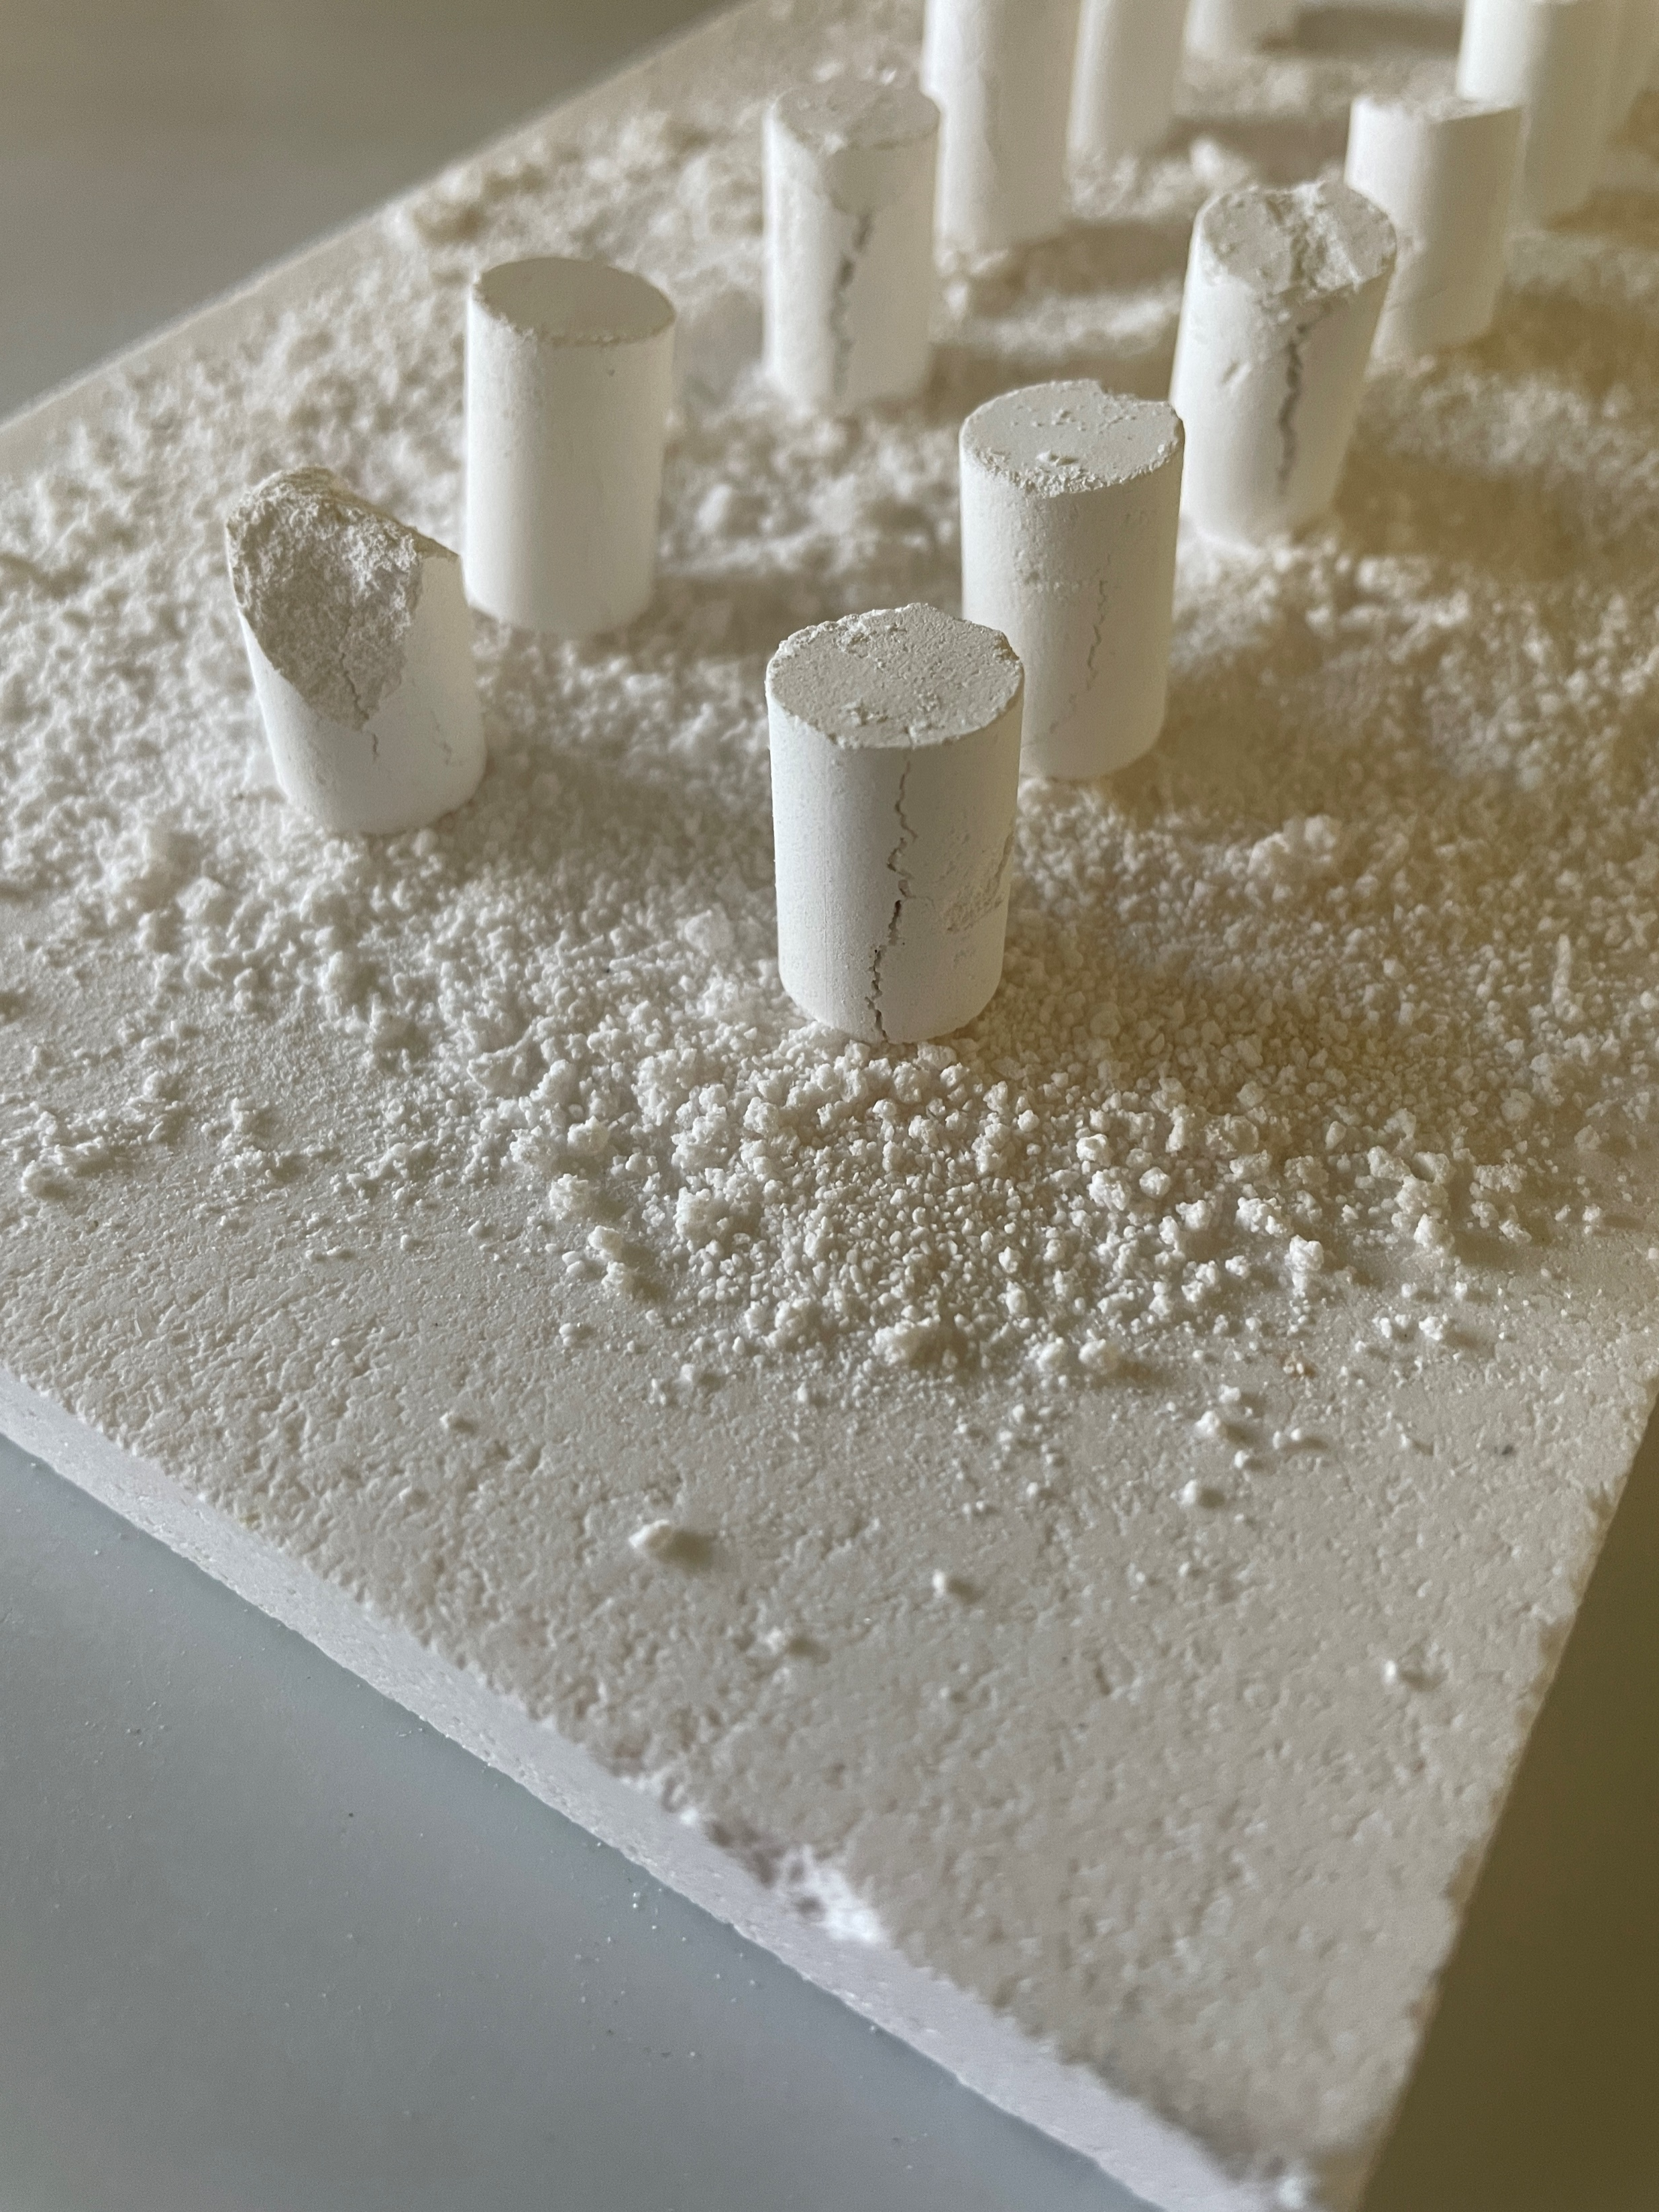
\includegraphics[width=0.333\columnwidth]{sample1.png} & 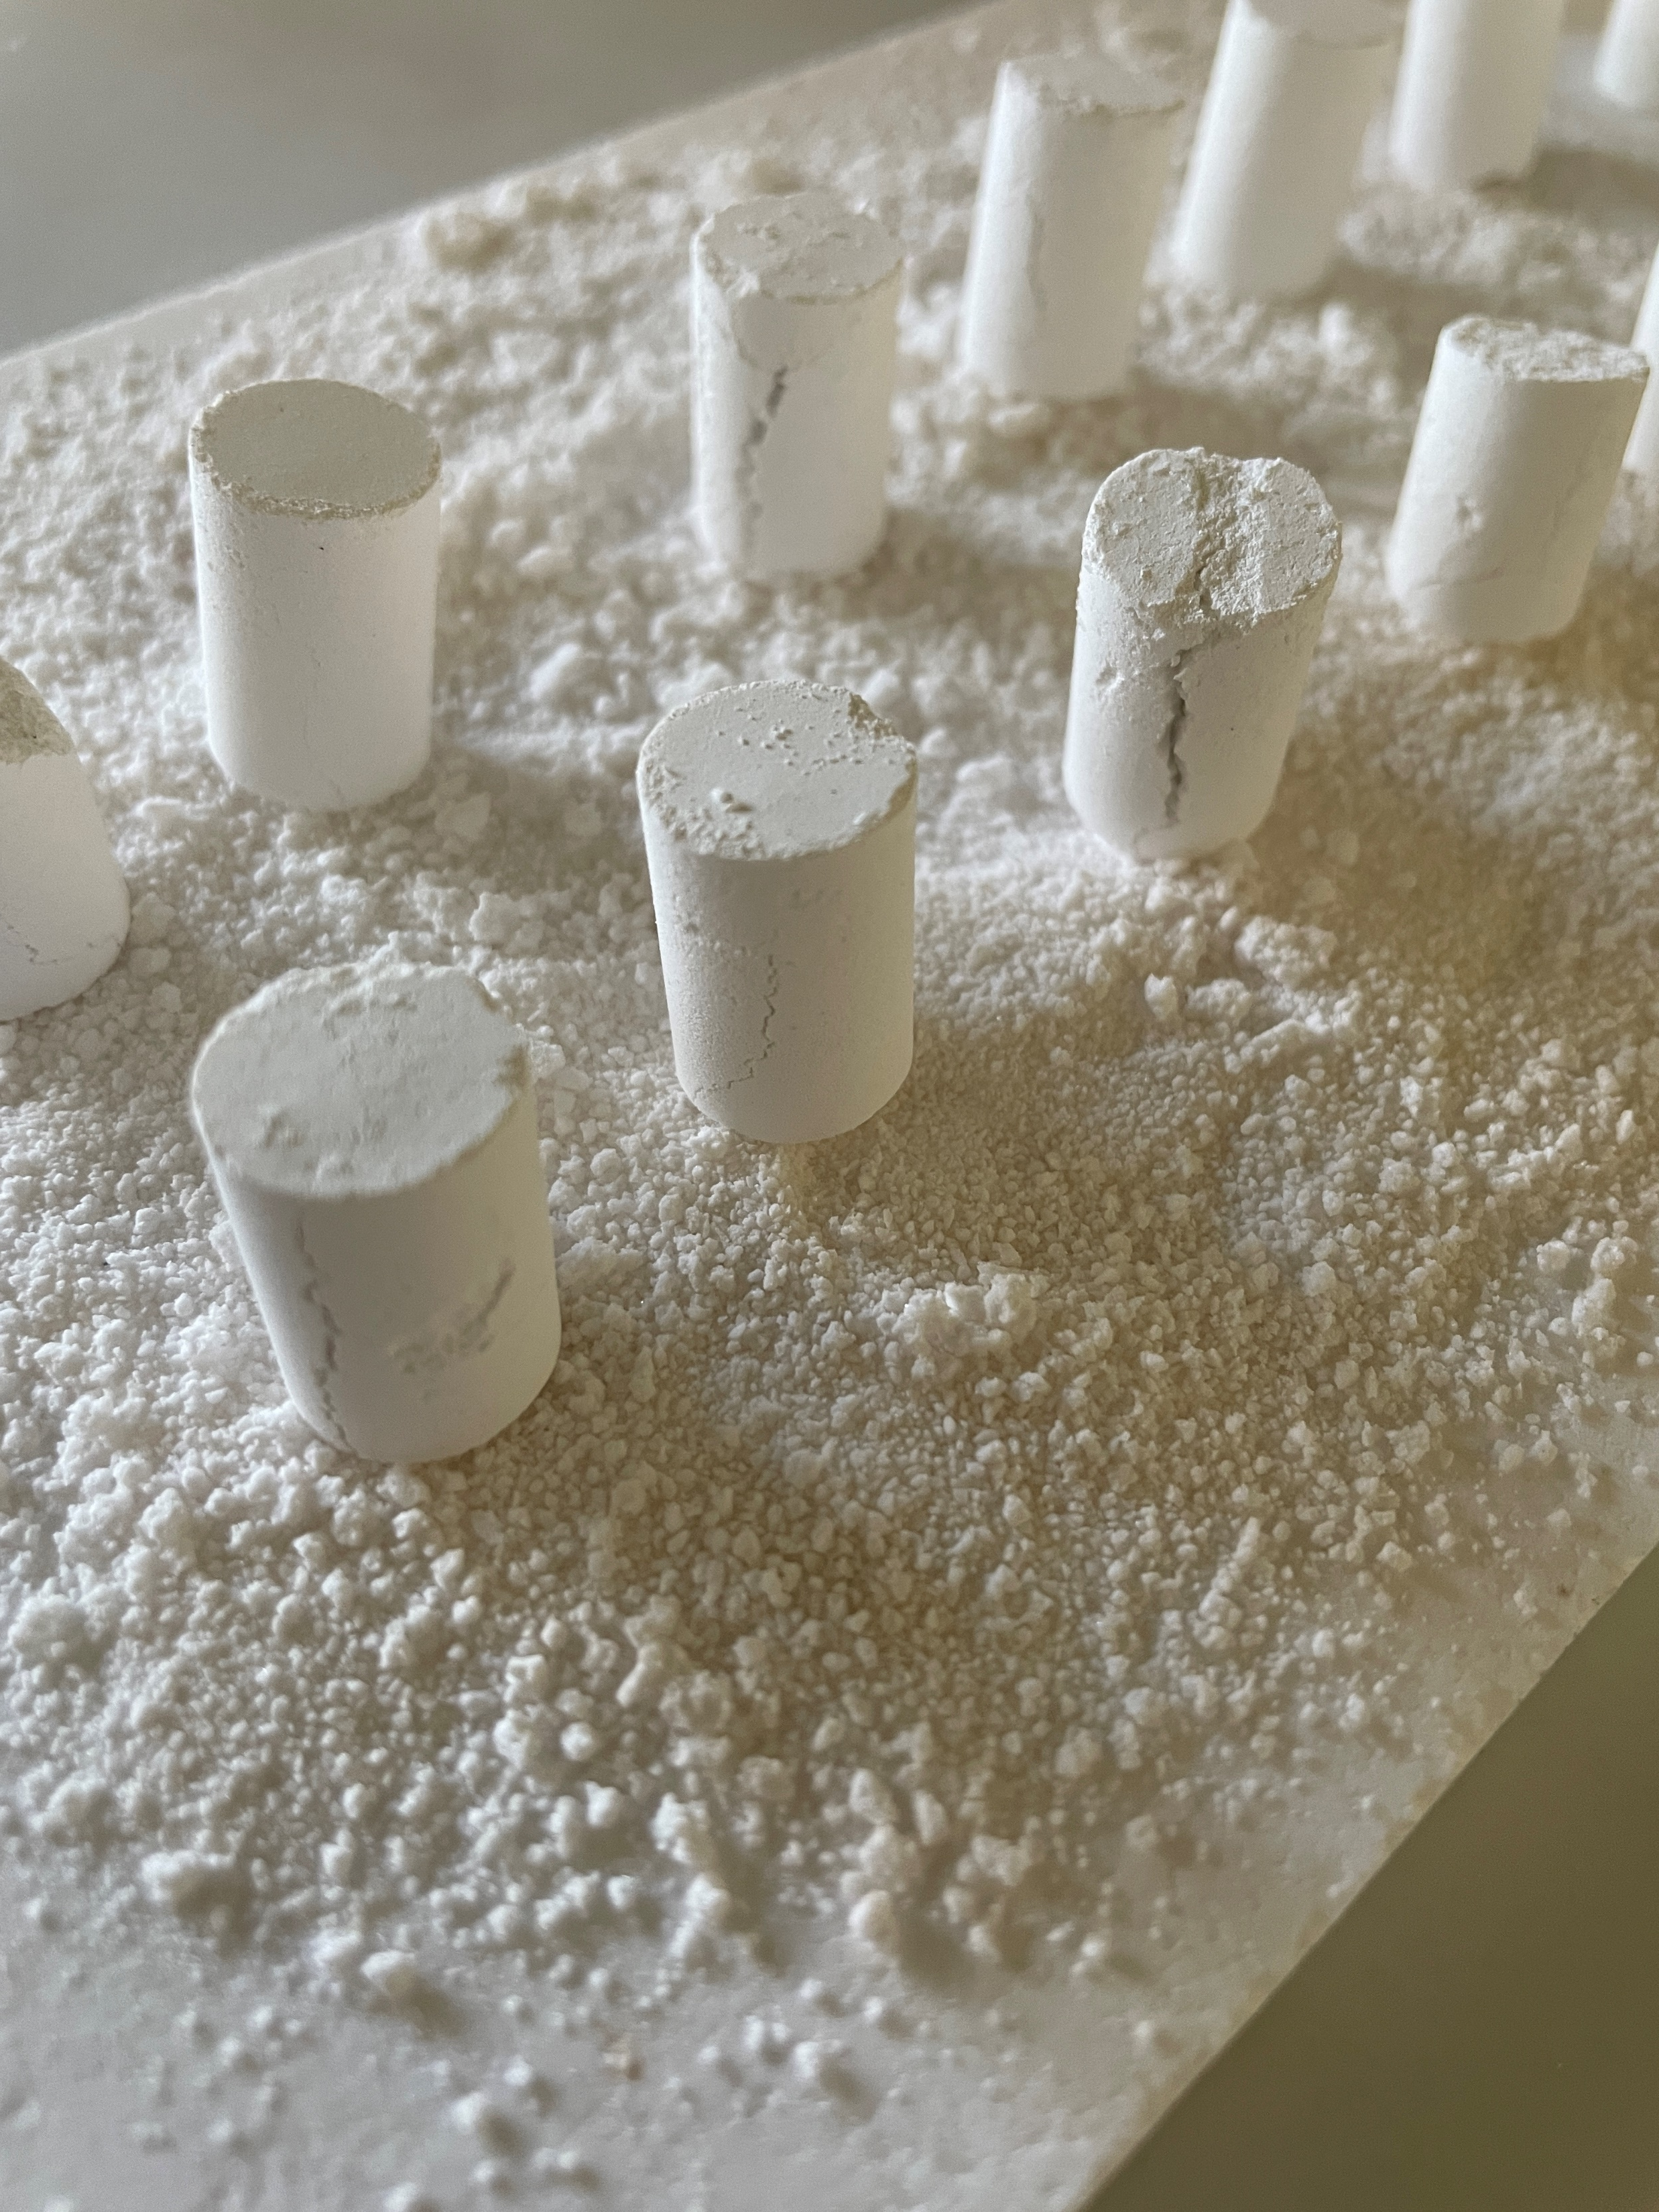
\includegraphics[width=0.33\columnwidth]{sample2.png} & 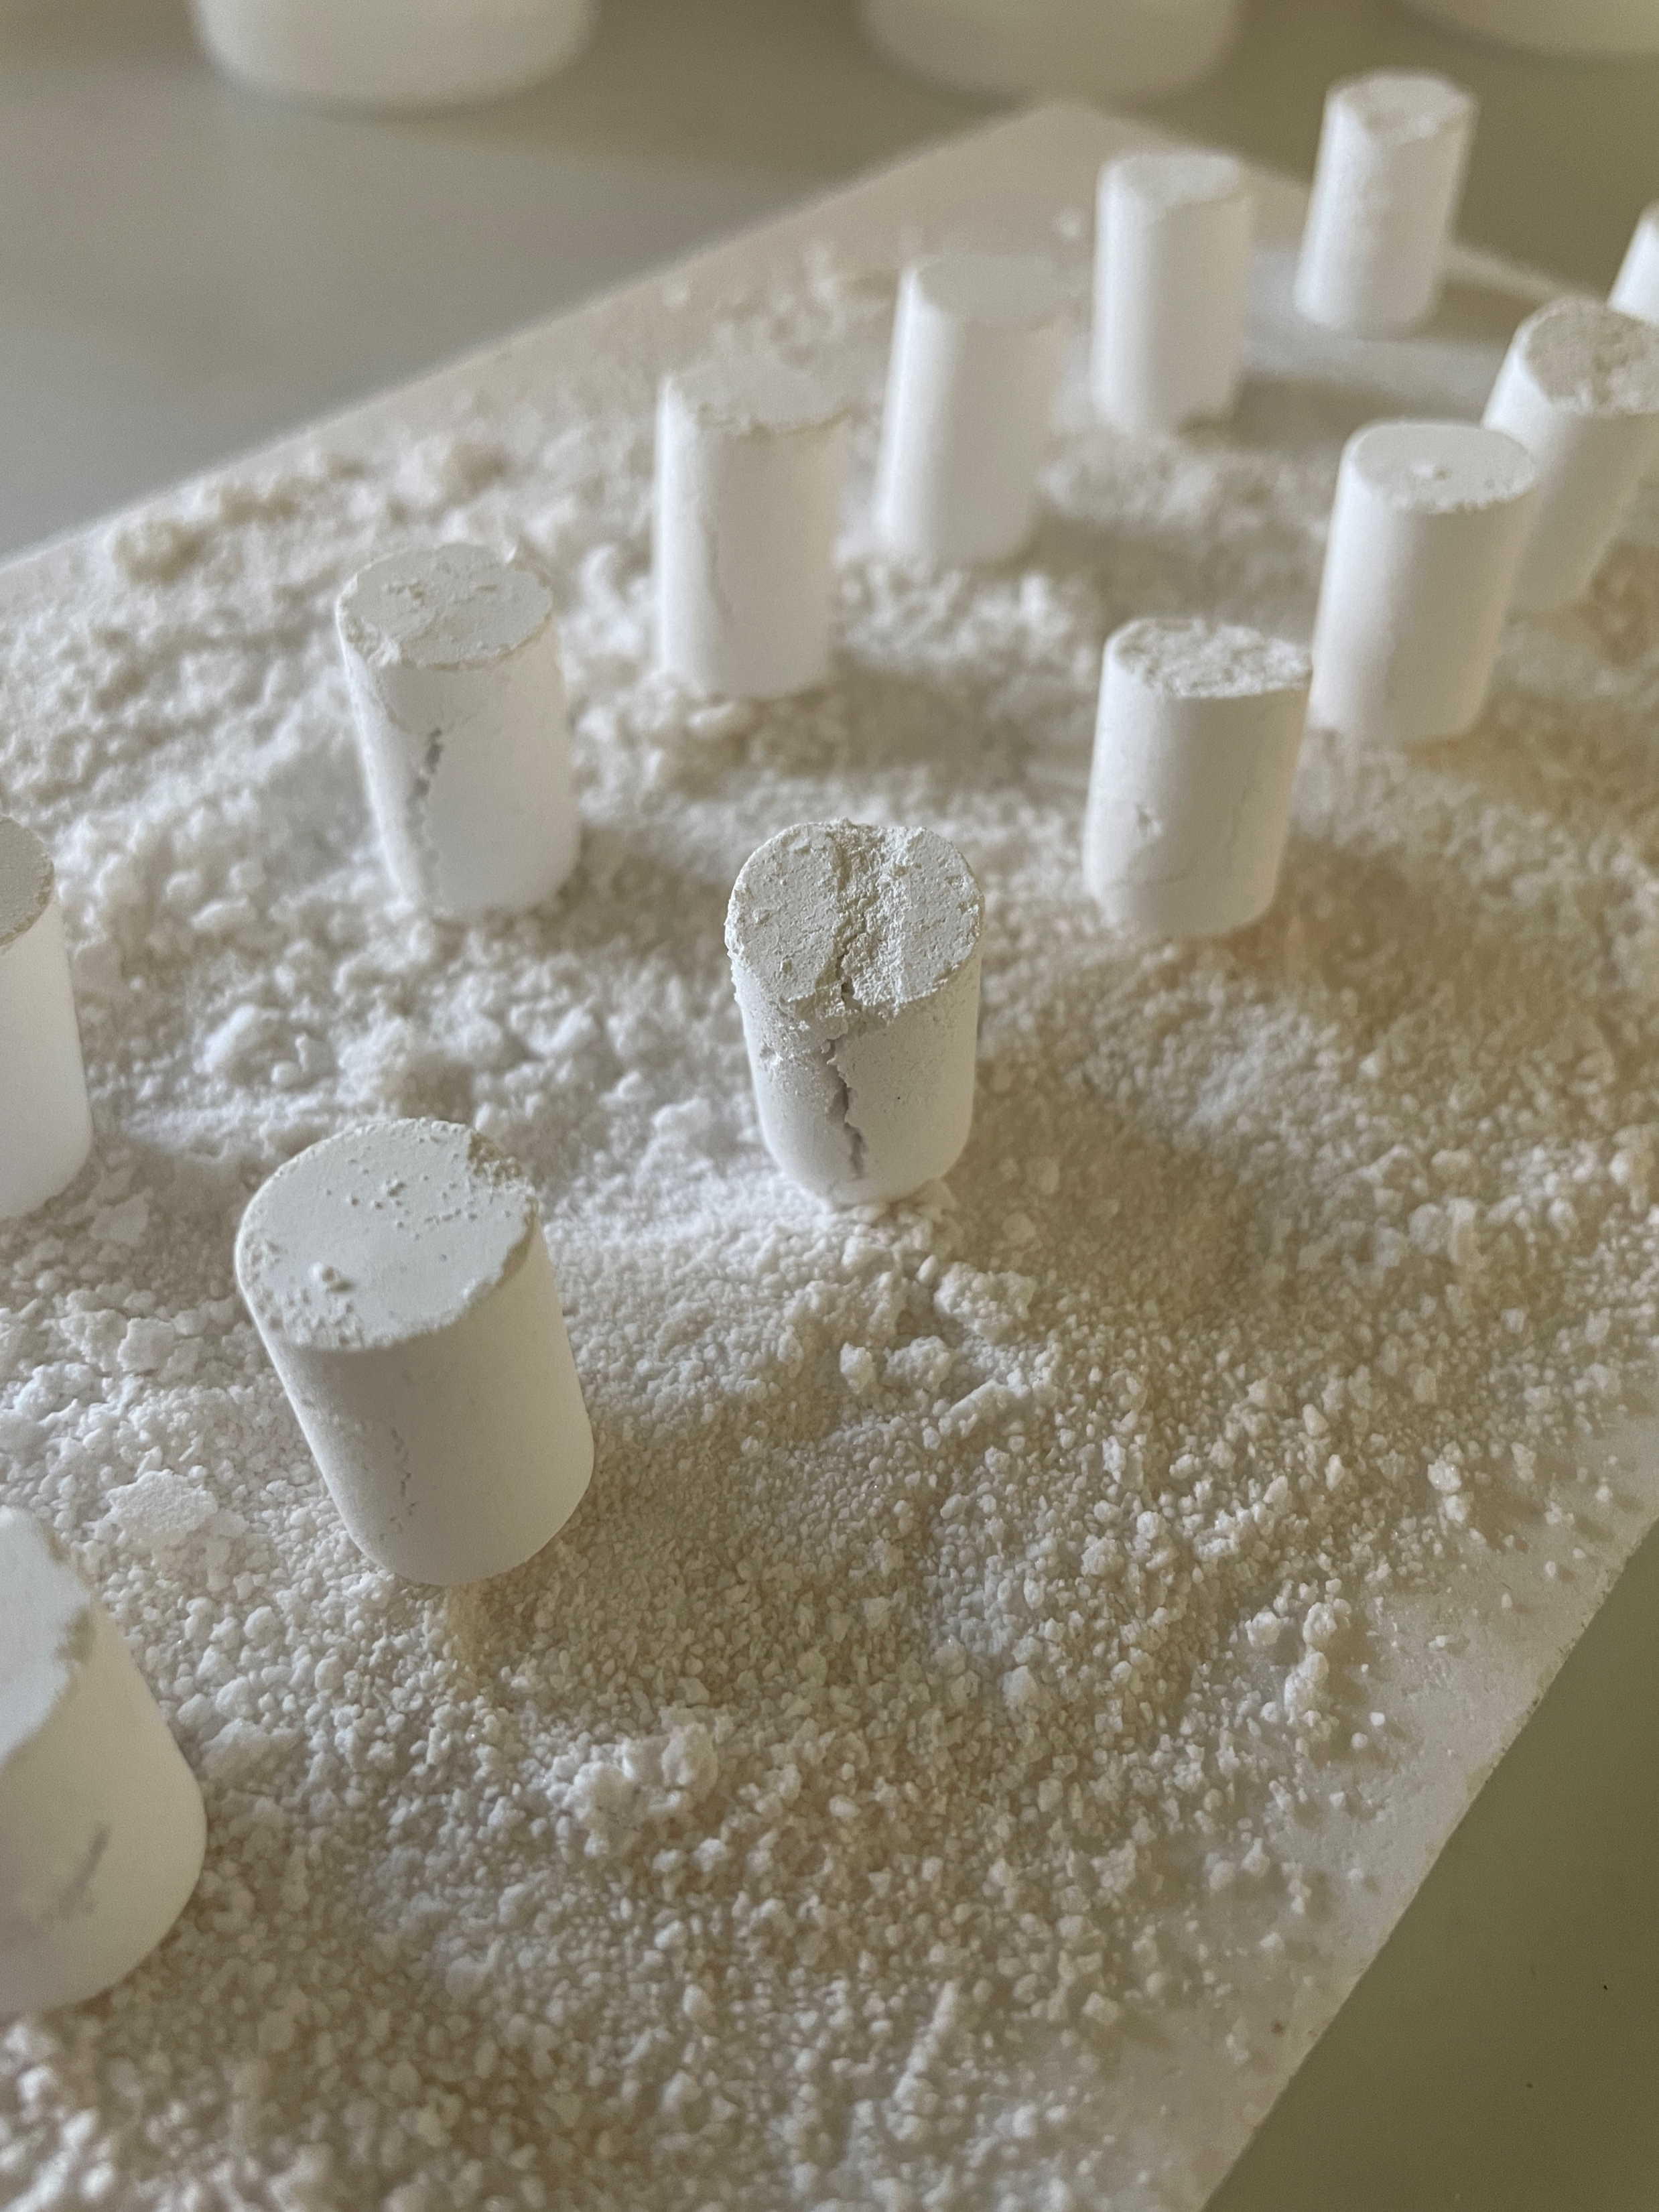
\includegraphics[width=0.33\columnwidth]{sample3.png} \\
%     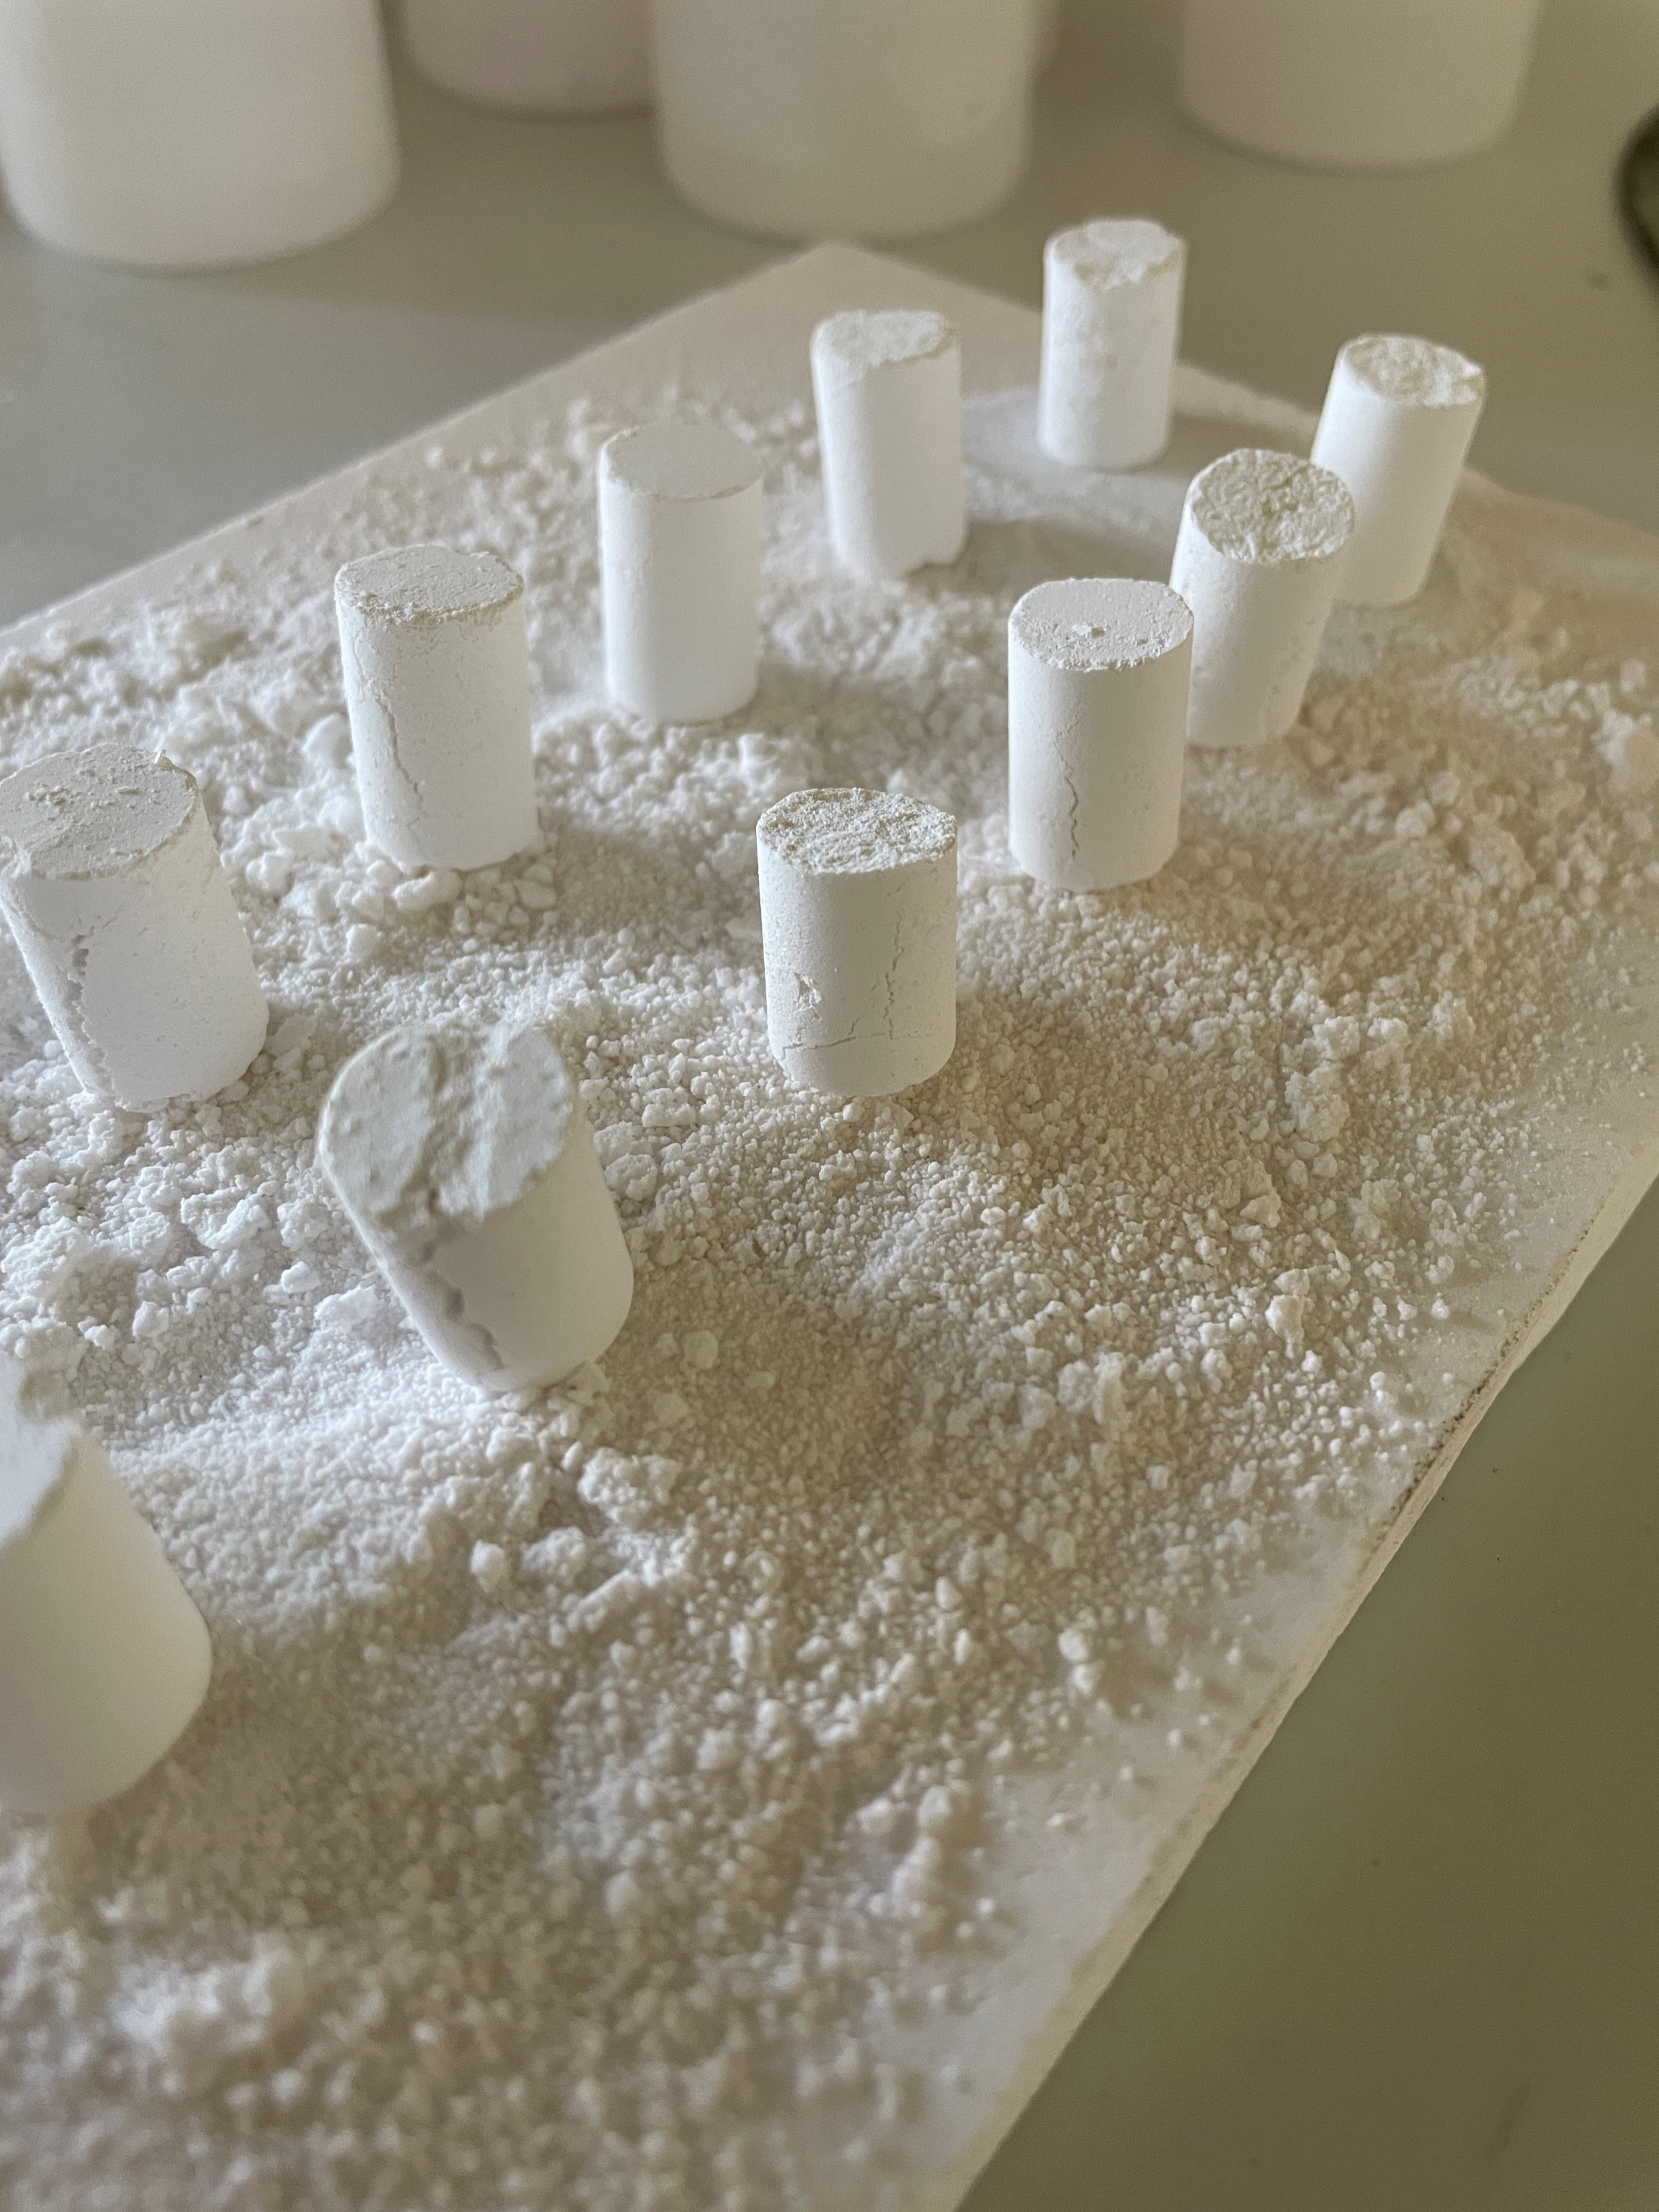
\includegraphics[width=0.333\columnwidth]{sample4.png} & 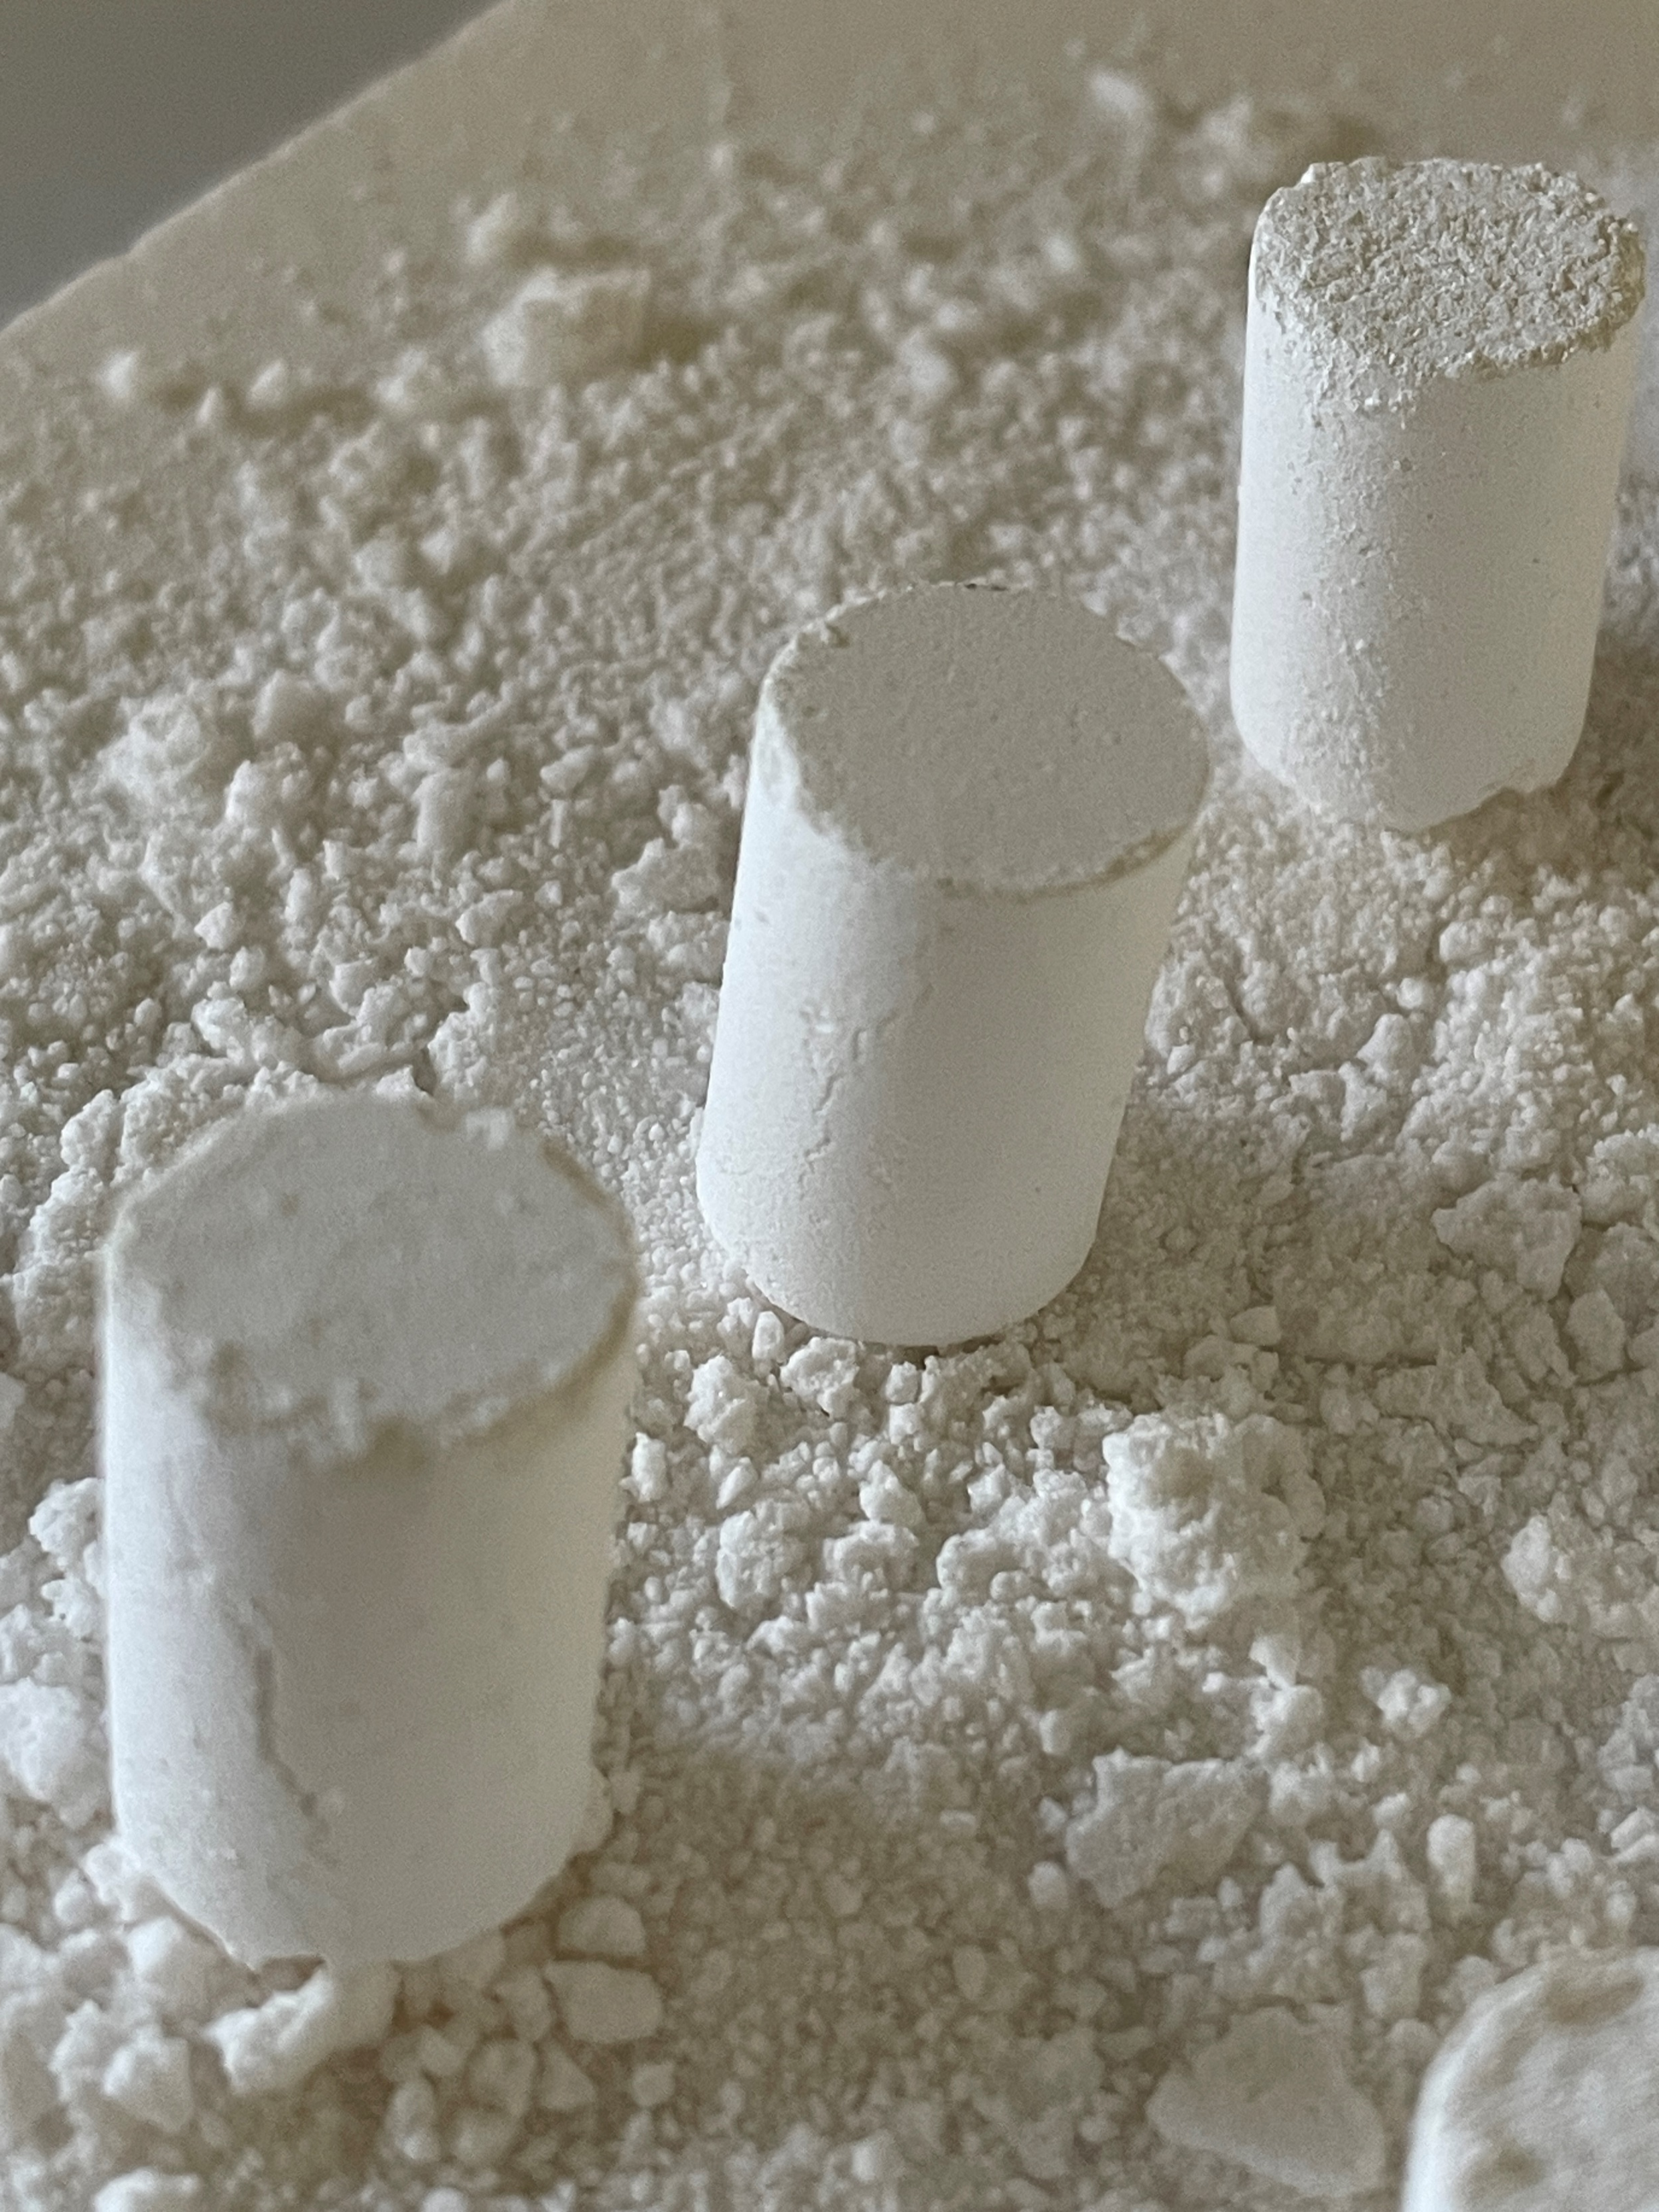
\includegraphics[width=0.33\columnwidth]{sample5.png} \\
%   \end{tabular}
%   \captionof{figure}{Result samples}
% \end{Figure}

\end{document}
